
\section{Kết luận}

\begin{frame}{Giải quyết các thách thức}
		\begin{itemize}
			\item Bằng việc dùng Cross-Local Attention và Self-Attention, chúng tôi giải quyết được quan hệ $1:n$ của cử chỉ và các điều kiện âm thanh, cảm xúc.
			\item Mô hình Diffusion giúp mô hình có thể học được các đặc trưng có phân bố dữ liệu thật thấp.
			\item Đảm bảo khả năng mở rộng (scalable) của hệ thống sinh cử chỉ để có thể ứng dụng trong thực tế.
		\end{itemize}
\end{frame}

\begin{frame}{Đóng góp chính}
	
	\begin{figure}
		\centering
		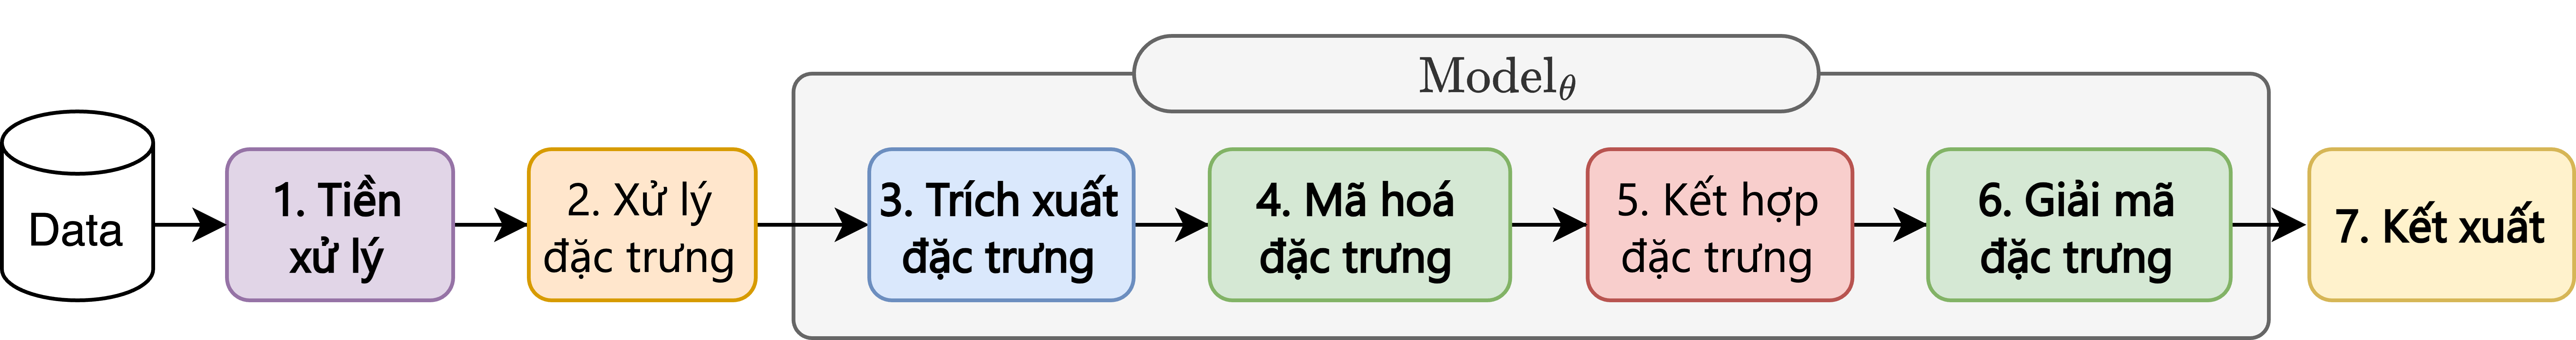
\includegraphics[width=0.9\linewidth]{TotalStage}
	\end{figure}
	
	\begin{itemize}
		\item Transcribe âm thanh để có được văn bản (\textit{Công đoạn tiền xử lý}, \textit{xử lý đặc trưng} và \textit{kết hợp đặc trưng}), làm dữ liệu bổ sung trong Diffusion có điều kiện.
		
		\item Mở rộng mã nguồn chương trình: \hyperlink{https://github.com/hmthanh/OHGesture}{\textbf{github.com/OHGesture}}, Mô hình pretrain: \hyperlink{https://huggingface.co/openhuman/openhuman}{\textbf{Huggingface.co/openhuman}}
		
		\item Giai đoạn Hệ thống trực quan hoá bằng Unity (\textit{Công đoạn Kết xuất}): \hyperlink{https://github.com/DeepGesture/deepgesture-unity}{\textbf{github.com/DeepGesture-Unity}}.
		
		\item Genea Leaderboard: Paper xây dựng hệ thống chuẩn hoá
		
		\item Đánh giá cử chỉ bằng FID: \hyperlink{https://github.com/GestureScore/GestureScore}{\textbf{github.com/GestureScore}}.
	\end{itemize}
\end{frame}

\begin{frame}[label=frame]{{Kết luận}}
	\begin{itemize}
		\item Mô hình \textbf{OHGesture}, có khả năng sinh cử chỉ chân thực, không chỉ trên các mẫu dữ liệu trong tập huấn luyện mà còn mở rộng được với những âm thanh không có trong dữ liệu huấn luyện.
		
		\item Sử dụng phương pháp \textbf{Classifier-free Guidance}, có thể điều khiển các điều kiện như cảm xúc, cử chỉ khởi tạo, có thể nội suy để suy luận ra giữa các cảm xúc khác nhau.
		
		\item Bài toán sinh cử chỉ còn rất mới, chúng tôi dự định sẽ dùng Fourier TT để trích xuất các đặc trưng về pha.
		
	\end{itemize}
	

%	In this slide, some important text will be
%	\alert{highlighted} because it's important.
%	Please, don't abuse it.
%	
%	\begin{block}{Remark}
%		Sample text
%	\end{block}
%	
%	\begin{alertblock}{Important theorem}
%		Sample text in red box
%	\end{alertblock}
%	
%	\begin{examples}
%		Sample text in green box. The title of the block is ``Examples".
%	\end{examples}
%	\hyperlink{appendix}{\beamerbutton{More on Appendix}}
\end{frame}